\subsubsection{\theoryC{The HL-LHC and HE-LHC Scope in Testing compositeness of 2HDMs}}
\contributors{S. De Curtis, L. Delle Rose, S. Moretti, A. Tesi, K. Yagyu}\rt{There are comments to address. HE-LHC luminosity should be 15/ab instead of 3/ab.}
%{\bf Author(s): S. De Curtis$^a$, L. Delle Rose$^{a}$, S. Moretti$^{b,c}$, A. Tesi$^{a}$, K. Yagyu$^{a,d}$}\\
%
%{\it \small $^a$INFN, Sezione di Firenze, and Department of Physics and Astronomy, University of Florence,} \\
%{\it \small Via G. Sansone 1, 50019 Sesto Fiorentino, Italy}\\
%{\it \small $^b$School of Physics and Astronomy, University of Southampton,} \\
%{\it \small  Highfield, Southampton SO17 1BJ, United Kingdom}\\
%{\it \small  $^c$Particle Physics Department, Rutherford Appleton Laboratory,} \\
%{\it \small  Chilton, Didcot, Oxon OX11 0QX, United Kingdom}\\
%{\it \small  $^d$ Seikei University, Musashino, Tokyo 180-8633, Japan} \\
%Ackn: SM is funded in part through the NExT Institute and the STFC CG ST/P000711/1.

%\subsubsection{Introduction}
%\paragraph*{Introduction}

Much has been written about the ability of TeV scale compositeness to naturally remedy the hierarchy problem of the Standard Model (SM),  in particular through the pseudo-Nambu Goldstone  boson (pNGB) nature of the Higgs state. This idea is borrowed from QCD: the discovered Higgs boson is the analogue of the pion.  Just like there are $\pi$, $\eta$, etc. mesons predicted by QCD, though, there could be several Higgs states predicted by compositeness beyond the one discovered. In this respect, a natural setting ~\cite{Mrazek:2011iu}   is the Composite 2-Higgs Doublet Model (C2HDM)~\cite{DeCurtis:2016scv,DeCurtis:2016tsm,DeCurtis:2017gzi}. It is built upon the experimentally established existence of a doublet structure triggering Electro-Weak Symmetry Breaking (EWSB),  generating the $W^\pm$, $Z$ and SM-like Higgs state $h$, yet it surpasses it by providing one more composite doublet of Higgs states that can be searched for at the LHC, alongside additional composite gauge bosons (the equivalent of the $\rho$, $\omega$, etc. of QCD) and 
composite fermions. We concentrate here on the Higgs sector of the C2HDM (see \citeref{DeCurtis:2018iqd} for a comparative study between the 2HDM based composite solution to the hierarchy problem and the one driven instead by Supersymmetry)    based on ${\rm SO}(6)\to {\rm SO}(4)\times {\rm SO}(2)$,  in presence of so-called {\sl partial compositeness}~\cite{Kaplan:1991dc} realised through the third generation of the SM fermions.  The scalar potential and, thus, the masses of the Higgs bosons are generated at one-loop level by the linear mixing between the (elementary) SM and the (composite) strong sector fields. This implies that masses and couplings are not free parameters, unlike in the elementary realisations, but they depend upon the strong sector dynamics  and are strongly correlated.
The compositeness scale $f$ is  within the energy domain of the LHC and  the composite nature of the SM-like Higgs boson in the C2HDM can  be revealed through corrections of ${\cal O}(\xi)$, where $\xi=v^2/f^2$, with $v$ being the \vev of the SM Higgs field. 
As current lower limits on $f$ are of order 800 GeV, this implies that such effects enter experimental observables at the 5-10\% level.
%Hence, it may reasonably be argued that the LHC might have problems in establishing them in the Higgs sector. \rt{Why? LHC has at least 10\% sensitivity in the Higgs sector no?}
%Indeed the ${\cal O}(\xi)$ corrections,  involving Yukawa interactions with top- and bottom-quarks or tau-leptons,  are notoriously difficult to measure at the LHC, as these lead to hadronic processes which are masked by the significant  QCD background present at the LHC. 
In order to test these effects, the best strategy is to probe gauge interactions of the SM-like Higgs boson, universally affected by ${\cal O}(\xi)$ corrections. In particular, these effects are expected to be larger than the correponding ones in Elementary realisations of a 2HDM (E2HDM)~\cite{Branco:2011iw}, and therefore accessible at the HL-LHC.  
However, if these were to be found consistent with those of the E2HDM, the last resort in the quest to disentangle the C2HDM from the E2HDM hypothesis would be to exploit the correlation among observable processes involving extra Higgs bosons.
Hence, under the above circumstances, it becomes mandatory to explore the scope of the HL- and HE-LHC, the latter being  necessary for processes involving Higgs boson self-interactions, which have  rather small cross-sections  at the current LHC, in exploring the structure of extended Higgs sectors.
We shall do so by studying under which LHC machine conditions one could access the processes $gg \to H \to hh \to b\bar b\gamma\gamma$ and $gg \to H\to t\bar t$ (followed by semi-leptonic top decays), as these will enable one to extract crucial C2HDM parameters, wherein $H$ is the heaviest of the two \cpeven (neutral) Higgs states of the C2HDM, the lightest ($h$) being the SM-like one.  

%\subsubsection{Numerical results}
%\paragraph*{Numerical results}

The construction of the model and the fundamental parameters of the C2HDM are described in \citeref{DeCurtis:2018iqd}. 
These correspond to the scale of compositeness $f$, the coupling of the spin-1 resonances, the masses of the heavy top partners, and the mixing between the latter and the elementary top quark (which represents the leading contribution to the effective scalar potential). 
% 
In order to have phenomenologically acceptable configurations with EW parameters consistent with data, we require: 
(i) the vanishing of the two tadpoles of the \cpeven Higgs bosons, (ii) the value of the top quark mass to match the measured one, 
and (iii) the value of the Higgs boson mass to match the measured one. 
Under these constraints, we explore the parameter space by scanning the scale of compositeness in the range $(600, 3000)$ GeV and all the other parameters in the range $(-10,10)f$.
%
As outputs, we obtain the masses of the charged Higgs boson $(m_{H^\pm})$, the \cpodd Higgs boson ($m_A$), and the heavier \cpeven Higgs boson ($m_H$), 
the mixing angle $\theta$ between the two \cpeven Higgs boson states ($h,H$), as well as their couplings to fermions and bosons. 
These quantities are then combined in physics observables and tested against experimental measurements through HiggsBounds~\cite{Bechtle:2013wla} and HiggsSignals~\cite{Bechtle:2013xfa},
which include {current} results from void Higgs boson searches and parameter determinations from the discovered Higgs state,
respectively. Further, we extrapolated the latter (at present counting on about 30 fb$^{-1}$ of accumulated luminosity after Run 1 and into Run 2) to 300 fb$^{-1}$ (end of Run 3) and 3000 fb$^{-1}$ (HL-LHC and HE-LHC), by adopting the expected experimental accuracies given in \citeref{CMS:2013xfa}  (scenario 2 therein).\rt{HE should be 15/ab} These are listed against the so-called 
$\kappa$'s (or `coupling modifiers')  of \citeref{LHCHiggsCrossSectionWorkingGroup:2012nn}, among which those interesting us primarily are $\kappa_{VV}^h$ ($V=W^\pm,Z$), $\kappa_{\gamma\gamma}^h$ and $\kappa_{gg}^h$, generally the most constraining ones.

Before proceeding with presenting our results, it is worth mentioning that a generic 2HDM Lagrangian 
introduces, in general, Flavour Changing Neutral Currents (FCNCs) at tree level via Higgs boson exchanges.
To avoid them, we assume here an alignment (in flavour space) between the Yukawa matrices like in the elementary Aligned 2HDM (A2HDM)~\cite{Pich:2009sp}. 
In this scenario, the coupling of the heavy Higgs $H$ to the SM top quark is controlled (modulo small corrections induced by the mixing angle $\theta \sim  \xi$) by
\begin{align}\label{eq:A2HDM}
\zeta_t=\frac{{\bar\zeta}_t-\tan\beta}{1+{\bar\zeta}_t\tan\beta},
\end{align}
where ${\bar\zeta}_t$ and $\tan\beta$ are predicted, and correlated to each other, in terms of the aforementioned fundamental parameters of the C2HDM.
Thus, being interested in the phenomenology of the $H$ state, henceforth we will map the results of our scan in terms of $m_H$ and $\zeta_t$ and restrict the parameter space to the region $m_{H,A,H^\pm} >2 m_h$.
The $\zeta_t$ parameter and the Higgs trilinear coupling $\lambda_{Hhh}$ set the hierarchy among the decay modes of the heavy state $H$. In particular, $H \rightarrow t \bar t$, when kinematically allowed, represents the main decay channel. Below the $t \bar t$ threshold, the diHiggs $H \rightarrow hh$ decay mode can reach, approximately, 80\%, with the remaining decay space saturated by $H \rightarrow VV$. 
The corresponding Branching Ratio (BR) observables are shown in \fig{fig:BRs} (left). Both of these can be notably different in the C2HDM with respect to the E2HDM, since the $Hhh$ and $Ht\bar t$ couplings can carry the imprint of compositeness (see  \fig{fig:BRs} (right) for their correlation).\rt{Can $v_{\text{SM}}$ be renamed $v$ in the figure?}
The hierarchy discussed above highlights the key role of the $H \rightarrow hh$ and $H \rightarrow t \bar t$ channels in the discovery and characterization of the composite heavy Higgs boson.
 \begin{figure}
\centering
{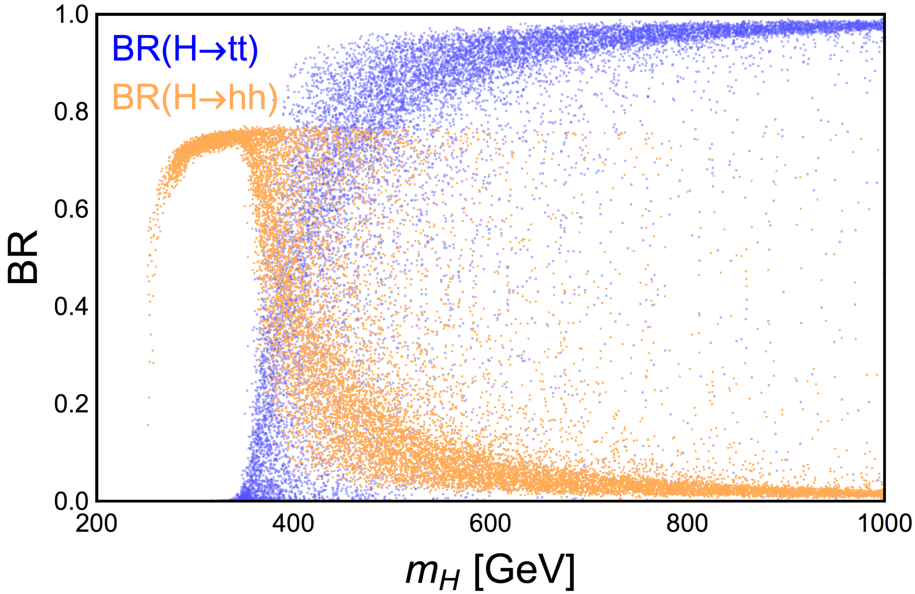
\includegraphics[scale=0.5]{\main/section7OtherSignatures/img/BRH-13TeV.pdf}} \quad
{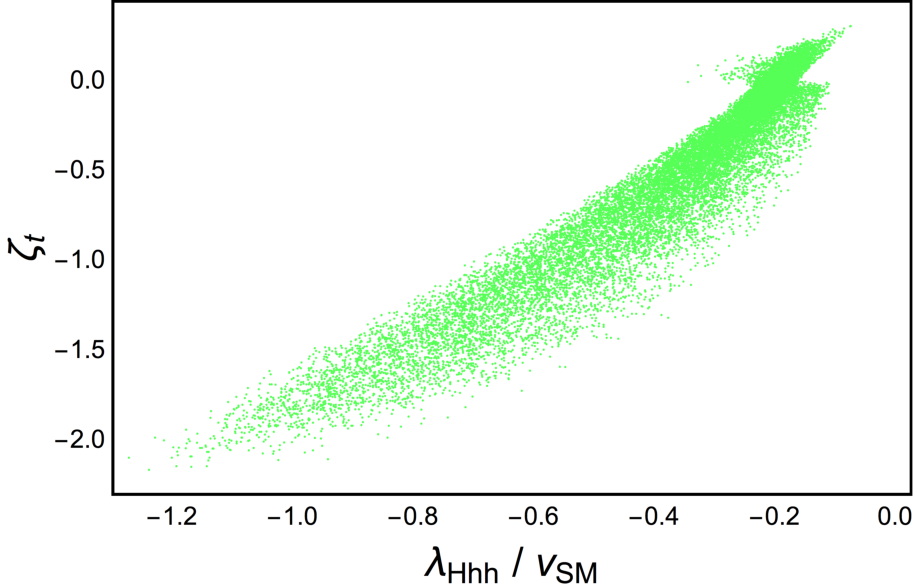
\includegraphics[scale=0.5]{\main/section7OtherSignatures/img/lHhh-zetaT.pdf}}
\caption{Branching ratio of the $H$ state of the C2HDM in the $hh$ (orange) and $t\bar t$ (blue) channels (left) and correlation between the $\zeta_t$ and $\lambda_{Hhh}$ couplings obtained upon imposing present HiggsBounds and HiggsSignals constraints at 13 TeV (right). 
\label{fig:BRs}}
\end{figure}


%
\begin{figure}
\centering
{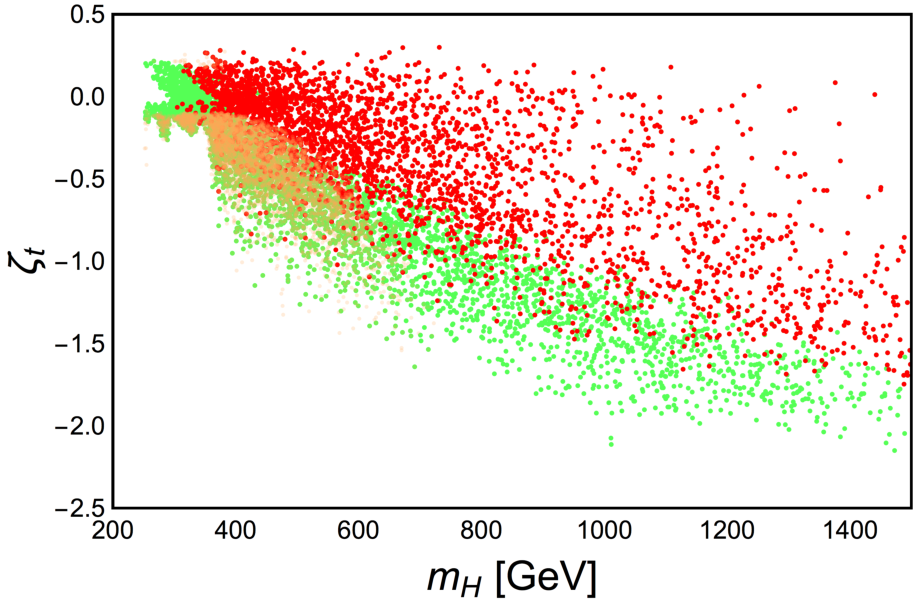
\includegraphics[scale=0.5]{\main/section7OtherSignatures/img/mA-zetaT_kVVkgg-bbgaga-L300.pdf}} \quad
{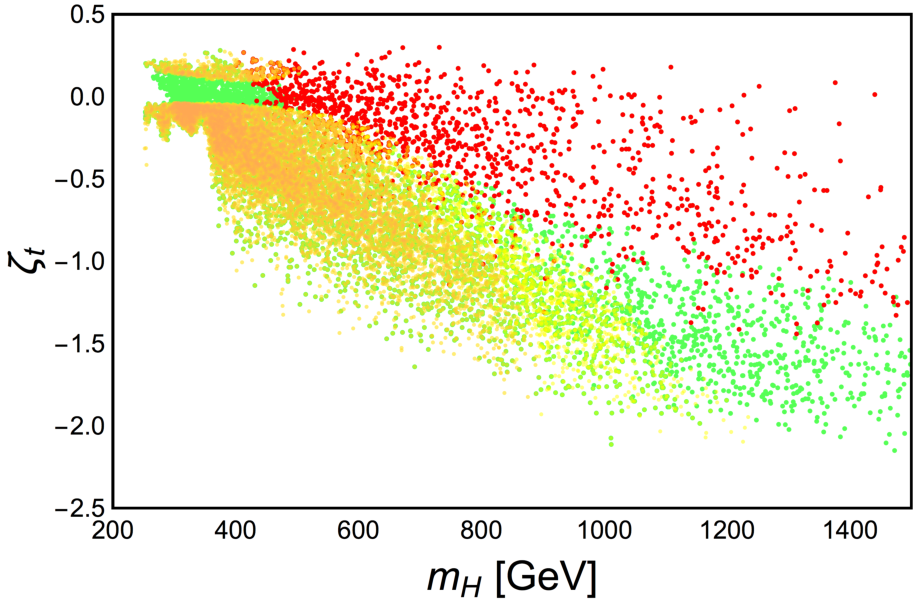
\includegraphics[scale=0.5]{\main/section7OtherSignatures/img/mA-zetaT_kVVkgg-bbgaga-27.pdf}}
\caption{Results of the C2HDM scan described in the text. Colour coding is as follows.
Green: all points that pass present constraints at 13 TeV. 
Red: points that, in addition to the above, have $\kappa_{VV}^h$, $\kappa_{\gamma\gamma}^h$ and $\kappa_{gg}^h$ within the 95\%~\cl projected uncertainty at $L=300$ fb$^{-1}$ (left) and $L=3000$ fb$^{-1}$ (right).
Orange: points that, in addition to the above,  are 95\%~\cl excluded  by the direct search $gg\to H\to hh\to b\bar b\gamma\gamma$, at $L=300$ fb$^{-1}$ (left) and $L=3000$ fb$^{-1}$ (right). In the right plot the yellow points are 95\%~\cl excluded by the same search  at the HE-LHC with $L=3000$ fb$^{-1}$.
\label{fig:bbgaga}}
\end{figure}

\begin{figure}
\centering
{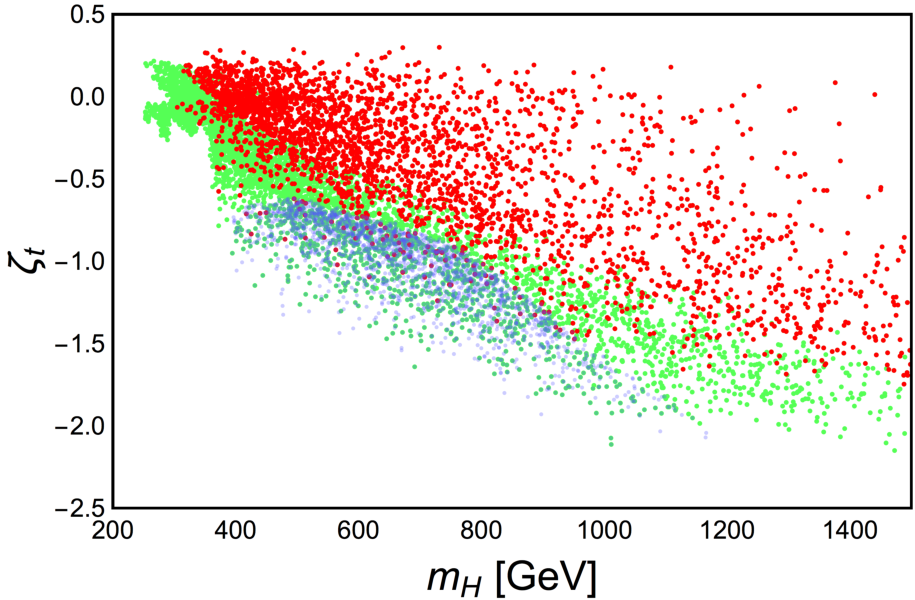
\includegraphics[scale=0.5]{\main/section7OtherSignatures/img/mA-zetaT_kVVkgg-tt-L300.pdf}} \quad
{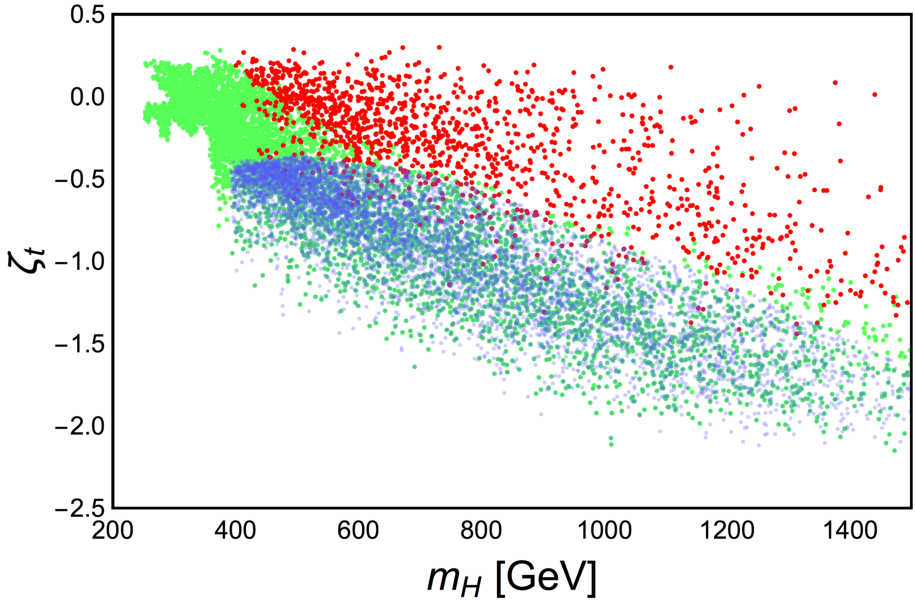
\includegraphics[scale=0.5]{\main/section7OtherSignatures/img/mA-zetaT_kVVkgg-tt-L3000.pdf}}
\caption{Green an red points are as in the previous plot.
Blue: points that, in addition to the above,  are  95\%~\cl excluded by  the direct search $gg\to H\to t\bar t$, at $L=300$ fb$^{-1}$ (left) and $L=3000$ fb$^{-1}$ (right).
\label{fig:tt}}
\end{figure}
Figures \ref{fig:bbgaga} and \ref{fig:tt} \rt{Is there any projection for HE in \fig{fig:tt}?} illustrate the interplay between direct and indirect searches and
the ability of the HL- and HE-LHC  to discover both the $gg\to H\to hh\to b\bar b\gamma\gamma$ and the $gg \to H\to t\bar t$ (followed by semi-leptonic top decays) signals, respectively, over regions of the C2HDM parameter space mapped onto the $(m_H,\zeta_t)$ plane, even when no deviations are visible in the aforementioned $\kappa$'s of the SM-like Higgs state $h$ (red points) at $L=300$ fb$^{-1}$ and $L=3000$ fb$^{-1}$. 
Notice that 95\%~\cl exclusion limits are extracted by  adopting the sensitivity projections of \citerefs{Aaboud:2018mjh} and~\cite{CMS:2017ihs} while compliance with the coupling modifiers is here achieved by asking that $|1 - k^h_i|$ is less than the percentage uncertainty declared in \citeref{CMS:2013xfa}, where $i=VV,\gamma\gamma$ and $gg$. Of some relevance, while tensioning the scope of the two search channels to one another, is to note that the orange  points have a large overlap with the red ones for small $| \zeta_t| $ values while 
the corresponding overlap of the blue region is smaller but it reaches larger $H$ masses. Hence, the first channel enables one to cover a larger C2HDM parameter space while the second one higher $H$ masses. Clearly, the combination of the two allows one to combine the benefits of either.  The  HE-LHC,  assuming $\sqrt s=27$ TeV and $ L=3000$ fb$^{-1}$,\rt{Should be 15/ab}  will improve the reach in the $H$ high mass region up to 1.2 TeV by studying the process $gg\to H\to hh\to b\bar b\gamma\gamma$. For the $gg \to H\to t\bar t$  channel,  the naive extrapolation of the sensitivity with the parton luminosities is unreliable because it is affected by the SM $t \bar t$ threshold effects.

In summary, both the HL- and HE-LHC display clear potential in accessing production and decay channels of the heavy \cpeven Higgs state of the C2HDM which can give direct access to key interactions that carry the hallmark of 
compositeness.
